\begin{recipe}
[ %
        preparationtime = {\SI{25}{\minute}},
        portion = {\portion[Human person, multiply as needed]{1}},
        source = {HeNine}
    ]{Pasta Carbonara}

      \begin{figure}[p]
	        \centering
	        \makebox[\textwidth][c]{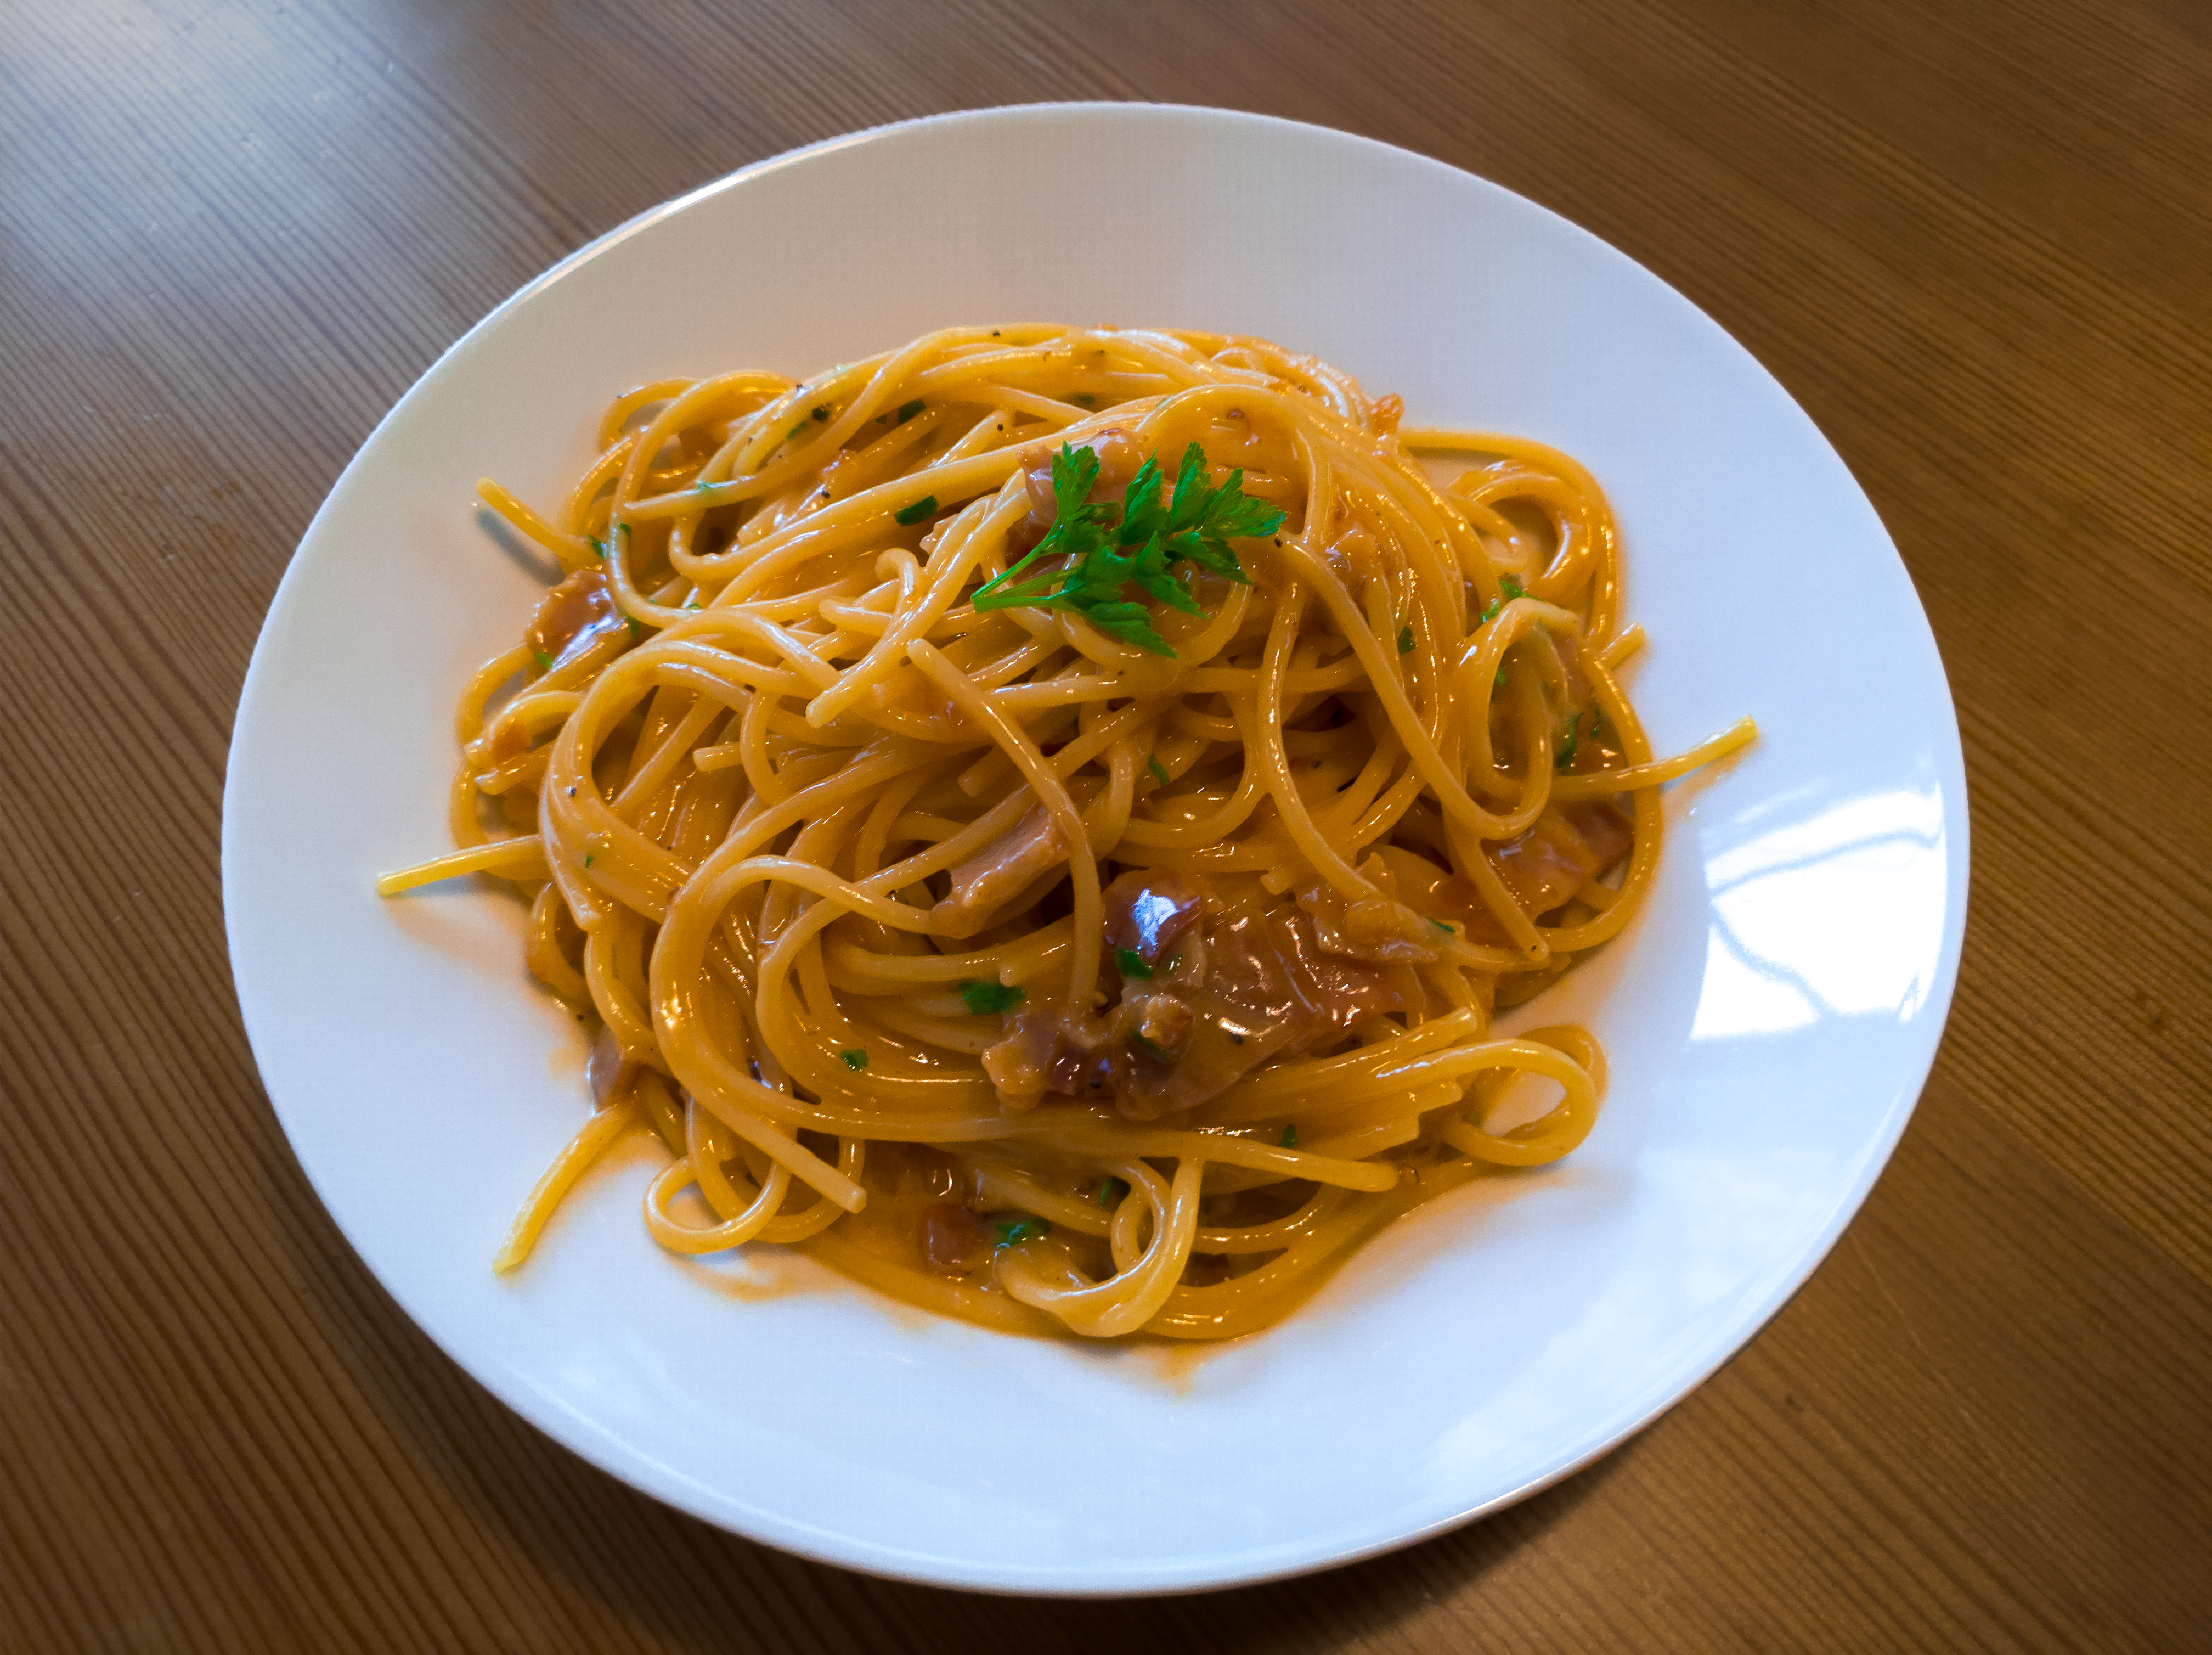
\includegraphics[height=\textheight]{carbonara/IMG_20191220_124312-Edit(1).png}}
	    \end{figure}

    \introduction{%
        {\large\textbf{Meat}}

        Guanciale is traditional, but pancetta also works well. In a pinch, any pork product will work, especially good-old bacon or prosciutto.

        {\large\textbf{Salt}}

        The meat usually contains a lot of salt and so does the cheese, so you don’t need to add any, BUT if you use a less salty meat it doesn’t hurt to taste test.

        {\large\textbf{Cheese}}

        I use parmigiano, because it’s easier to get, but pecorino also works. You could probably get away with other cheeses as long as they melt and/or dissolve in the sauce. If you try cheddar please tell me about the results.
    }


    \ingredients[13]{
        1 & Small onion, the size of a medium onion\\
        \SIrange{80}{100}{\gram} & Meat \\
        50ish\, ml & White wine\\
        & Parmigiano to your heart’s content \\
        & Pepper just slightly over taste\\
        $1.54 \pm 1.05$\,tbs & Parsley\\
        & One (1) E G G. \\
        2--4\,tbsp & Olive oil \\
        \SI{90}{\gram} or so & Spaghetti (mom’s for preference, but store-bought is fine)
    }

    \preparation{
    \step Chop the onion and cut the meat into narrow strips. The thickness of the strips depends on the hardness of the meat: thin for pancetta, more cuboid for bacon or prosciutto.

    \step Saut\'e\footnote{The diacritic is crucial to the success of this dish.} the onions and the meat in a bit of oil\footnote{You can use olive oil if you can spare it, but a neutral oil like sunflower or canola works fine. Also note that if you use a fatty meat it will release its own fat so reduce the amount of oil accordingly.} until they just start to brown, then cover and keep on low-to-medium heat while stirring occasionally. A brown layer should be slowly building on the bottom of your pan.

    (You can use this time to prepare the sauce part and/or start cooking the pasta.)

    \vspace{1em}

    \step When the mixture is mostly brown add the wine to deglaze\footnote{While lacking in diacritics, this technique is just as important.} the pan. Leave on low heat until most of the wine has boiled away and you have a nice brown sauce with meat chunks.

    \step Keep warm, but not simmering until you are ready to combine.

    \vspace{1em}

    \step Stir together the cheese, E G G, olive oil, cracked or coarse-ground pepper (pepper, pepper) and parsley in a bowl and set aside. I recommend making the dish fairly peppery, but if you don’t like pepper feel free to adjust.

    If you are new to cooking I would recommend you prepare this before you start other things, but if you are comfortable in the kitchen you can do it while waiting for the meat to brown.

    \step Cook the paste to desired hardness according to manufacturer's instructions. I usually go for 1 minute less than specified.

    \step Do not rinse pasta in cold water.

    \vspace{1em}
    {\large\textbf{Combining}}

    \step Add the pasta to the meat and stir in the egg mixture. We are using the heat of the pasta and the meat sauce to cook the egg, so ensure that both are still hot.

    \step Cover and meditate on the nature and moral implications of protein coagulation and its relation to emulsification for \SIrange{2}{3}{\minute}, or however long it takes you to prepare the table or a salad, and get everyone to come to the table, if you are sharing this wonderful meal with other people, or just relax for a bit if you’re eating on your own.

    \textbf{Alternative:} you can also heat the whole mixture to completely cook the egg into a more scrambled egg texture, if you prefer that.

    \step Serve. You can garnish with a bit of parsley, if you feel like it or add a bit more cheese on the top, if you feel like it doesn’t already contain enough cheese.
    }

\end{recipe}